\chapter{Einleitung}
In der vorliegenden Arbeit wird eine zweidimensionale diskrete Fouriertransformation in VHDL implementiert. Diese Tätigkeit erfolgt im Rahmen des Projekts \gls{isar} an der 
Hochschule für angewandte Wissenschaften Hamburg.
 \section{Motivation}
 Bisherige Analysen und Versuche wurden überwiegend auf theoretischer Ebene mit der Simulationssoftware Matlab oder anhand einer ca. 7x7\,cm großen Sensormatrix mit 64 einzelnen Sensoren in Verbindung mit
 einem an den PC angeschlossenen Microkontroller vorgenommen. Auf diese Weise können reale Messwerte ermittelt und verschiedene Szenarien getestet werden.
 
 Das Ziel des ISAR-Projekts ist, einen \gls{asic} zu fertigen, auf dem die Sensoren und alle Berechnungen erfolgen. 
 zunächst ist die Entwicklung der signalverarbeitenden Komponenten in einer Hardwarebeschreibungssprache geplant.
 Ziel ist ein Sensormodul, mit dem eine kontinuierliche Winkelberechnung zur Positionsbestimmung möglich ist. Dieses soll beispielsweise die Rotorlage eines Elektromotors ermitteln und die Information als digitales Nutzsignal ausgeben können. Ein wesentliches Aspekt ist das Unterdrücken von Störfeldern, welche in Form von Inhomogenitäten, unter anderem hervorgerufen durch Fehlpositionierung (Ablage) und Schrägstellung des Gebermagneten und den Magnetsensoren selbst, verursacht werden. 

 Den erste Schritt der Signalverarbeitung stellt die Berechnung der zweidimensionalen dirketen Fouriertransformation der Sensorsignale dar (Abb. \ref{pic:AblaufFourier}), da sich im Fourierraum Störanteile leichter filtern lassen. 
 Derzeit ist offen, ob anschließend der Winkel direkt berechnet werden kann oder vorher eine Rücktransforation erfolgen muss.
 

\begin{figure}[ht!]
 \centering
 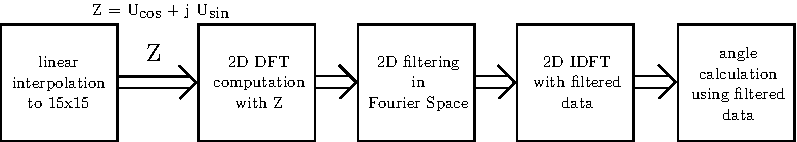
\includegraphics[width=0.8\textwidth]{img/AblaufFourier.pdf}
 \caption{Ablauf der Signalvorverarbeitung~\autocite[9]{krrts2017freqfilt}}
 \label{pic:AblaufFourier}
\end{figure}


\section{Stand der Technik}

Zur Winkelberechnung auf Basis von Magnetsensoren lassen sich verschiedene Effekte nutzen. Als erstes gelang es Sensoren auf Basis des Hall-Effekts zu entwickeln. Fortschreitende Technik ermöglichte es, die schon länger bekannten Effekte \gls{amr2}, \gls{gmr2} und aktuell \gls{tmr2} herzustellen. Sensoren die den TMR-Effekt nutzen gibt es bereits seit mehreren Jahren, es werden aber weitere Fortschritte angestrebt und erzielt. 
Die Entwicklung von Sensoren die die verschiedenen magnetoresistive Effekte nutzen, bringen Vorteile hinsichtlich des Strombedarfs, der Amplitude des Sensorsignals, Genauigkeit der Auflösung, Größe sowie benötigte Feldstärke~\autocite[2]{magSensTechOverview}. Darüber hinaus ist es nur mit den GMR- und TMR-Sensoren möglich 360${}^\circ$ aufzulösen. Die AMR-Sensoren erzeugen je Umdrehung zwei Sinusschwingungen, wodurch eine um 180${}^\circ$ versetzte Doppeldeuigkeit entsteht~\autocite{tsukakoshi2017tmrgmr}. Bei Hall-Sensoren sind die anderen genannten Schwächen deutlich stärker ausgeprägt, weswegen sie in diesem Bereich keine Verwendung finden.



%Der verwendete Prozess ist mit $\SI{350}{nm}$ im Vergleich zu modernen Prozessen mit $\SI{20}{\nm}$ oder weniger Strukturbreite um den Faktor 20 größer. Entsprechend handelt es sich um einen relativ alten Prozess.

%Kurze Beschreibung zu Standardzellen.


\section{Ziel dieser Arbeit}
Um eine Aufwandsabschätzüng einer 2D-DFT bezüglich Rechendauer und Flächenbedarf als Komponente auf einem  \gls{asic} zu erlangen, wird die Transformation auf ein Array angewandt, welches eine Größe 
hat, die sich leicht optimieren lässt. Herauszufinden, auf welche das Zutrifft, ist Teil der Arbeit. 
Es sollen Grundlagen erarbeitet werden, welche für die Transformation einer
15x15-Matrix nützlich sind. Letztere wird durch lineare Interpolation der 8x8-Sensormatrix errechnet (Abb. \ref{pic:AblaufFourier}). Von ihr ist bekannt, dass sie wegen einer vergleichsweise hohen Anzahl verschiedener Faktoren bedeutend
aufwändiger zu implementieren ist, weshalb zunächst mit einer einfacheren Berechnung Erfahrungen gesammelt und Vorarbeit geleistet werden soll.
Nach Möglichkeit soll für beide Matrixmultiplikationen, die die 2D-DFT mit der Twiddlefaktormatrix erfordert, die selbe DFT-Einheit genutzt werden. Herauszufinden, ob und wie dies effizient erfolgen kann,
gehört ebenfalls zur Aufgabenstellung.
